\section{Getting Started}

\subsection{About Version Control}
\begin{frame}[t]{Local Version Control System}
  \begin{center}
    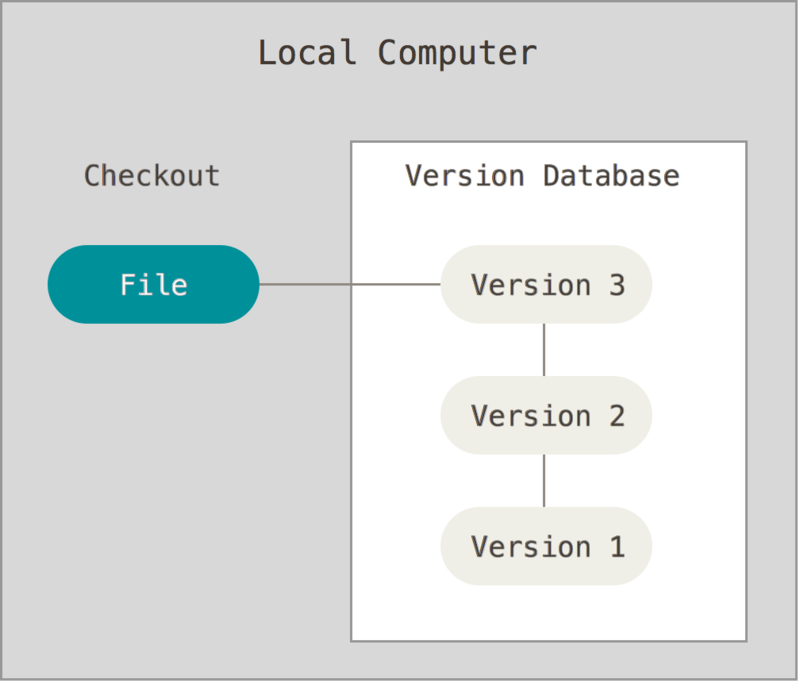
\includegraphics[height=2.75in]{../images/02-getting-started/local}
  \end{center}
\end{frame}

\begin{frame}[t]{Centralized Version Control Systems}
  \begin{center}
    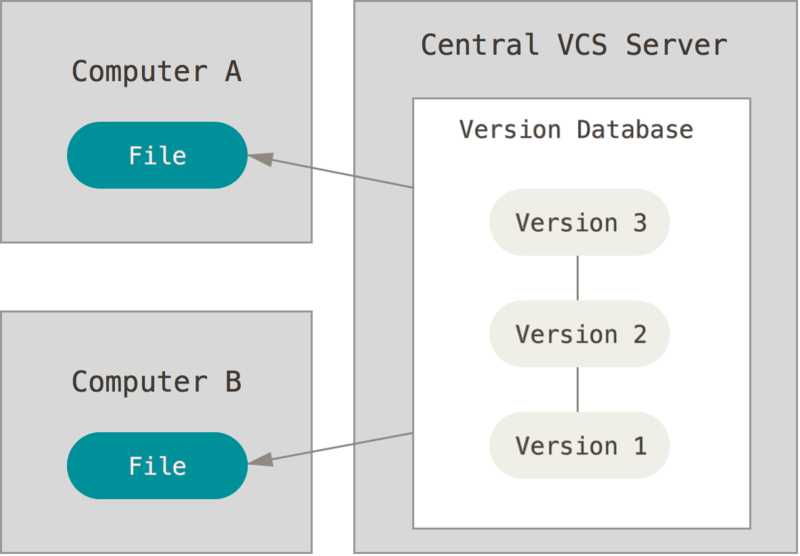
\includegraphics[height=2.75in]{../images/02-getting-started/centralized}
  \end{center}
\end{frame}

\begin{frame}[t]{Distributed Version Control Systems}
  \begin{center}
    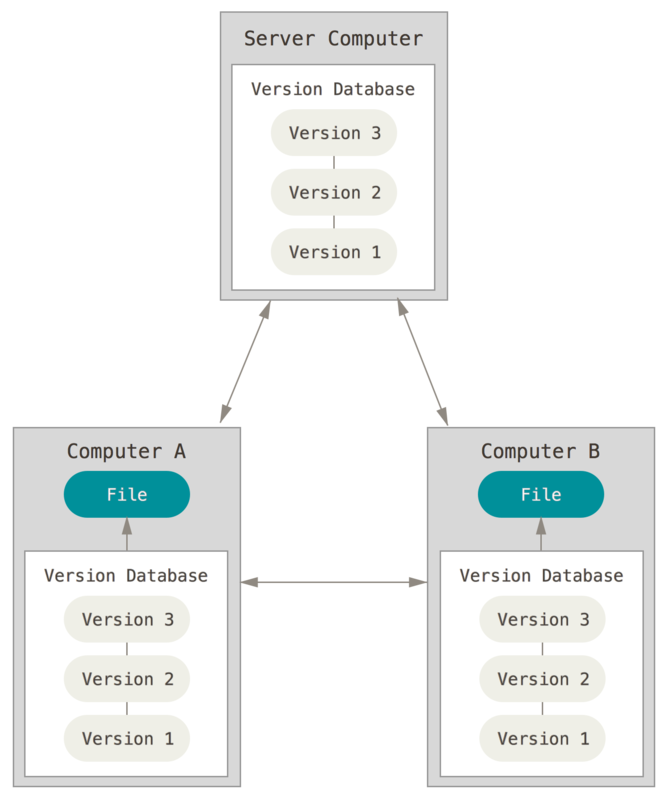
\includegraphics[height=2.75in]{../images/02-getting-started/distributed}
  \end{center}
\end{frame}

\subsection{A Short History of Git}
\begin{frame}[t]{Short History of Git}
  \begin{itemize}
    \item Linux (Linus Torvalds) vs BitKeeper
    \item 2005: Linux development community sets out to develop their own DVCS
      with goals for the new system of
      \begin{itemize}
        \item speed,
        \item simple design,
        \item strong support for non-linear development (thousands of parallel
          branches),
        \item fully distributed, and
        \item albe to handle large projects, like the Linux kernel,
          efficiently.
      \end{itemize}
  \end{itemize}
\end{frame}

\subsection{Git Basics}
\begin{frame}[t,allowframebreaks]{Snapshots, Not Differences}

  The Subversion model: file-based changes.

  \begin{center}
    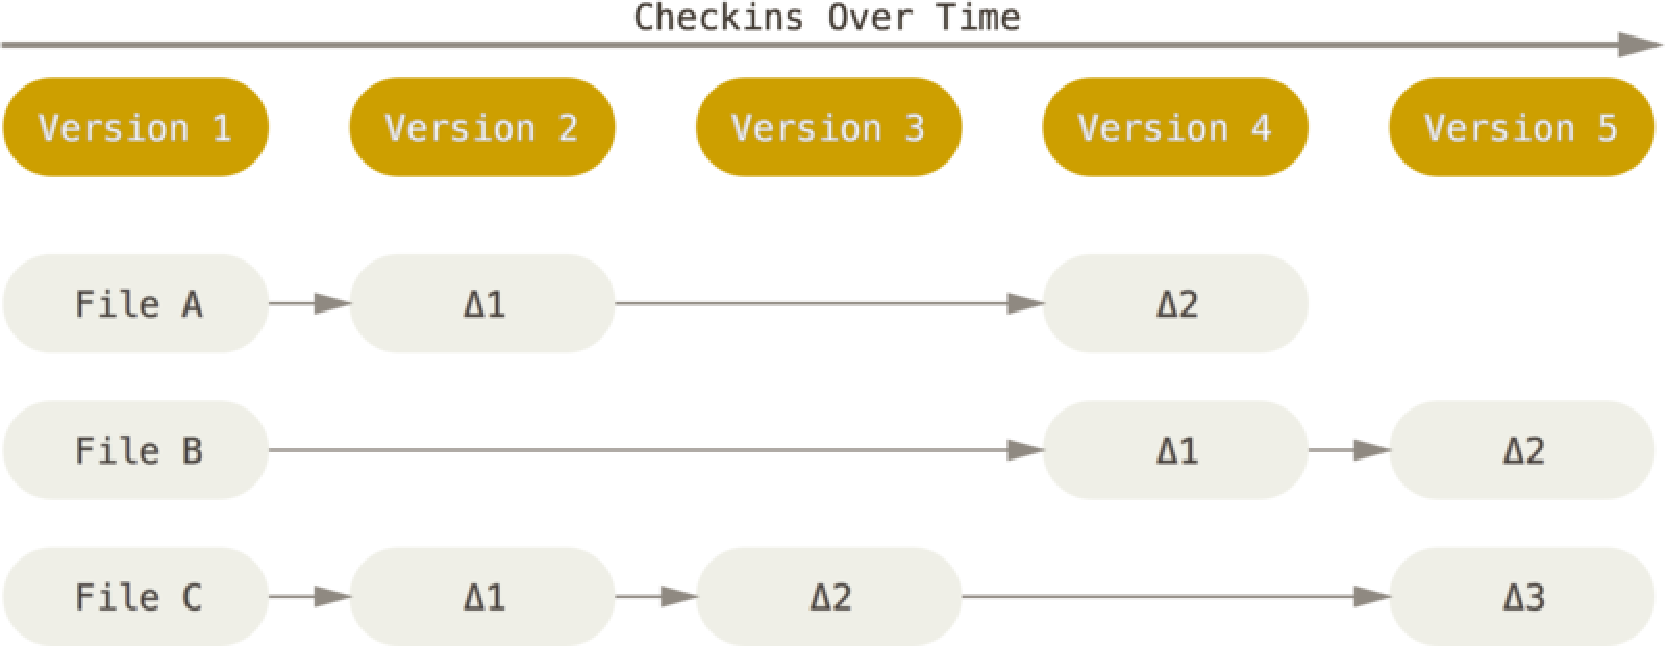
\includegraphics[width=0.98\textwidth]{../images/02-getting-started/deltas}
  \end{center}

  \pagebreak

  The Git model: a stream of snapshots.

  \begin{center}
    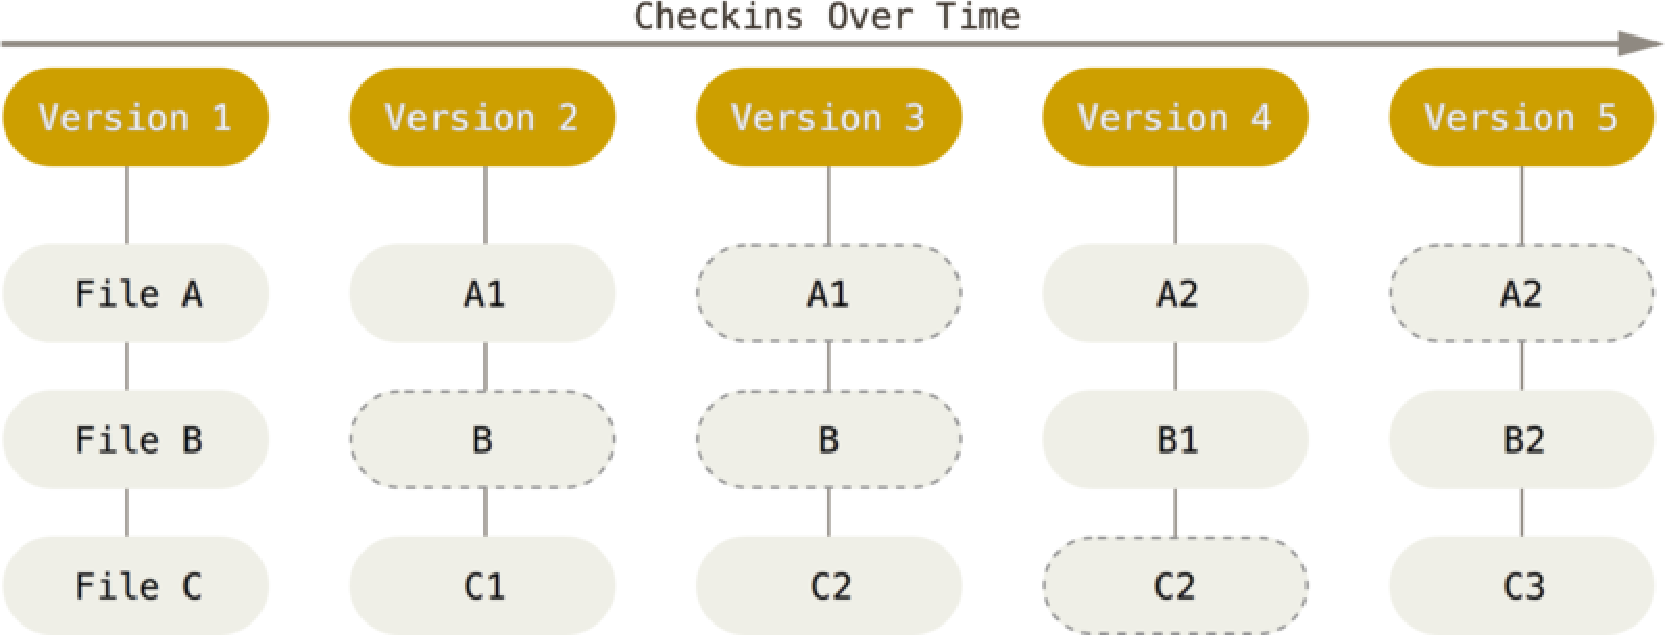
\includegraphics[width=0.98\textwidth]{../images/02-getting-started/snapshots}
  \end{center}

\end{frame}

\begin{frame}[t]{Nearly Every Operation is Local}
  \begin{itemize}
    \item Most operations are local.
      \begin{itemize}
        \item No need to talk to other computers on a network.
        \item The entire project history is on your local disk.
      \end{itemize}

    \item You can work offline.
    \item You can work off VPN.  
  \end{itemize}
\end{frame}

\begin{frame}[t]{Git Has Integrity}
  \begin{itemize}
    \item Everything is check-summed (remember the sha?)
    \item You can't lose informatin in transit nor get a file corruption without
      Git being able to detect it.
    \item Git stores everything in its database not by file name but by the hash
      value of its contents.
  \end{itemize}
\end{frame}

\begin{frame}[t]{Git Generally Only Adds Data}
  \begin{itemize}
    \item 
  \end{itemize}
\end{frame}

\begin{frame}[t]{The Three States}
\end{frame}

\subsection{The Command Line}
\begin{frame}[t]{}
\end{frame}

\subsection{Intalling Git}
\begin{frame}[t]{}
\end{frame}

\begin{frame}[t]{}
\end{frame}

\begin{frame}[t]{}
\end{frame}

\begin{frame}[t]{}
\end{frame}

\begin{frame}[t]{}
\end{frame}

\begin{frame}[t]{}
\end{frame}

\begin{frame}[t]{}
\end{frame}

